% pages: [visual, visual]
\documentclass[20pt,a4paper,landscape]{extarticle}
\usepackage[margin=1.45cm,top=0.45cm,left=0.9cm,right=0.9cm,bottom=0.9cm]{geometry}
\usepackage{amsmath}
\usepackage{amssymb}
\usepackage{graphicx}
\usepackage{xcolor}
\usepackage[sfdefault,lf]{FiraSans}
\renewcommand{\familydefault}{\sfdefault}
\setlength{\parindent}{0pt}
\pagestyle{empty}
\everymath{\displaystyle}
\begin{document}
\sffamily
\boldmath
{\LARGE \textbf{Time — Proficient}}\par\vspace{0.35em}
\begin{center}
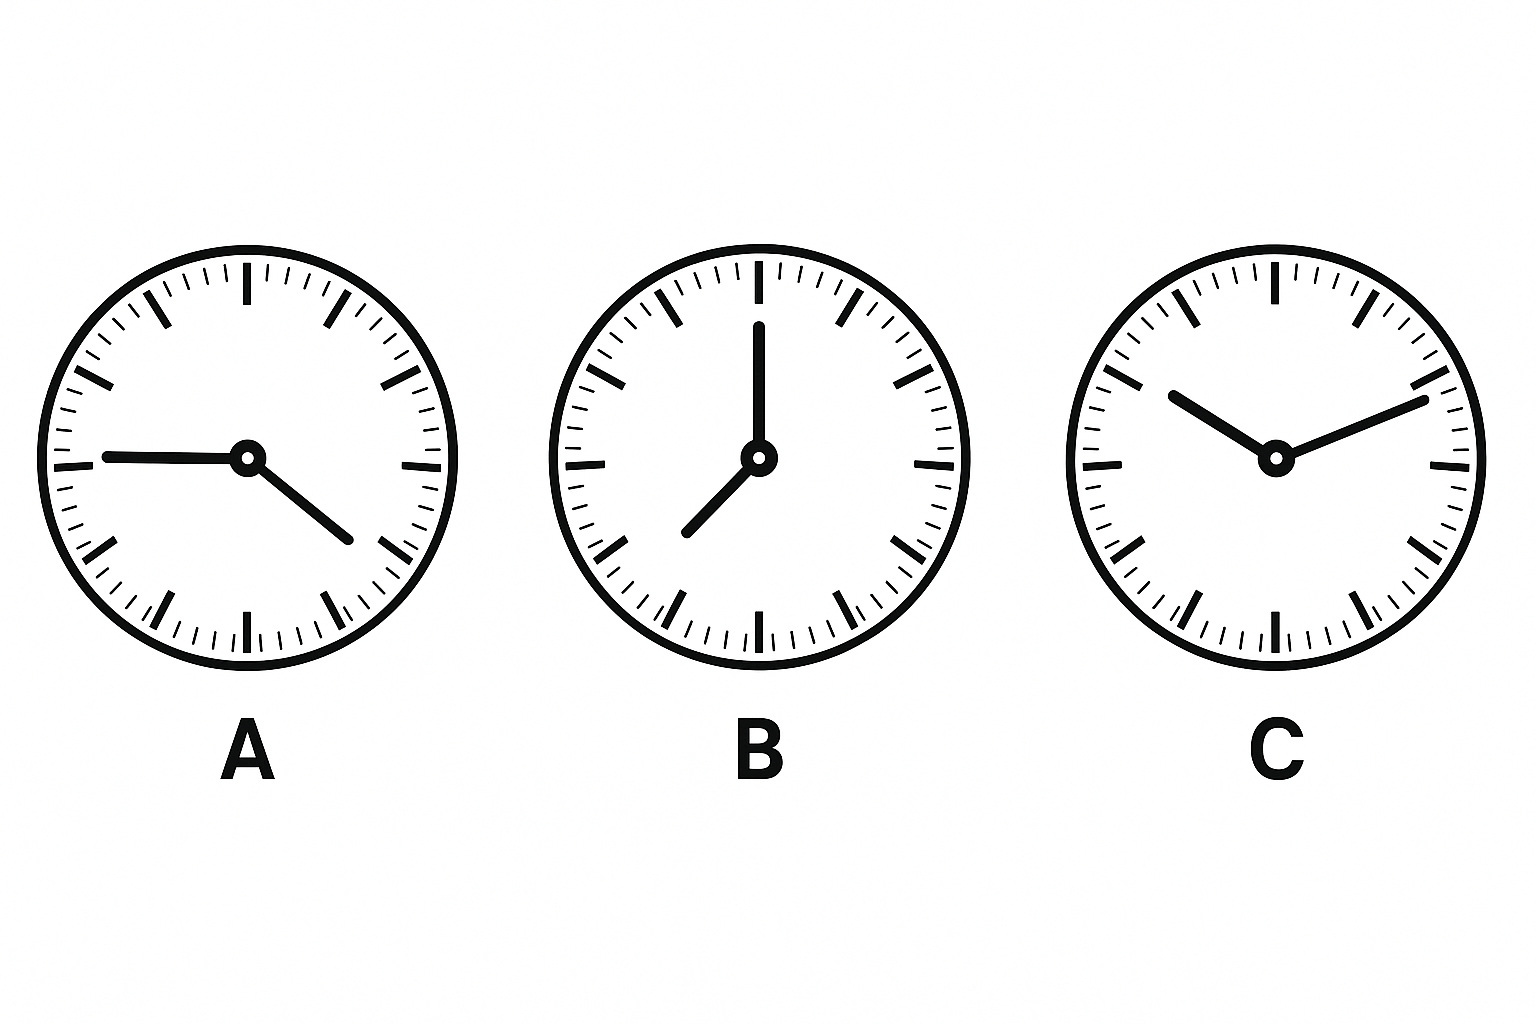
\includegraphics[width=0.94\linewidth,height=0.49\textheight,keepaspectratio]{web-diagrams/proficient-time-composite.png}
\end{center}
\vspace{0.35em}
% Questions referencing the image above
\noindent\begin{minipage}[t]{0.30\linewidth}\vspace{0pt}\textbf{1.} Read clock A. Write the time in words and in digital 24-hour format.\end{minipage}\hspace{0.05\linewidth}\begin{minipage}[t]{0.30\linewidth}\vspace{0pt}\textbf{2.} Read clock B. What is the time 35 minutes later? Write your answer in analogue terms and digital format.\end{minipage}\hspace{0.05\linewidth}\begin{minipage}[t]{0.30\linewidth}\vspace{0pt}\textbf{3.} Read clock C. A train departs at the time shown and takes 2 hours 15 minutes. What time does it arrive?\end{minipage}\par

\vspace{1.0em}
\begin{center}
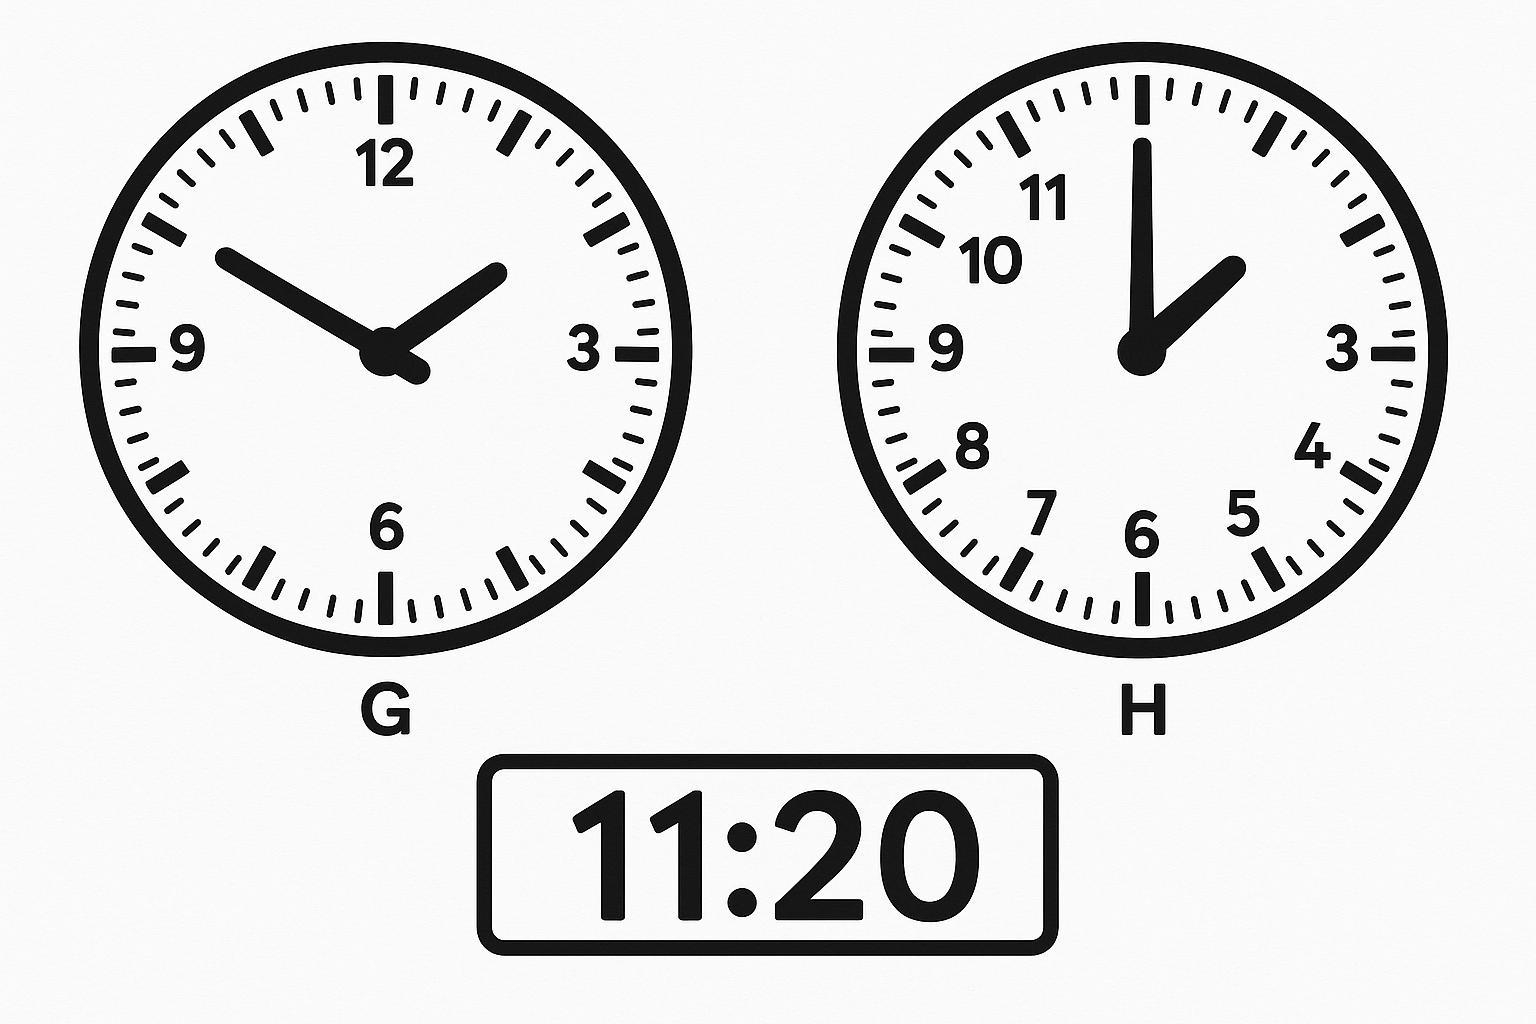
\includegraphics[width=0.94\linewidth,height=0.49\textheight,keepaspectratio]{web-diagrams/proficient-time-page2-diff.png}
\end{center}
\vspace{0.35em}
% Page 2 visual questions (time differences)
\noindent\begin{minipage}[t]{0.30\linewidth}\vspace{0pt}\textbf{4.} Read clock G and clock H. What is the time difference between G and H in hours and minutes?\end{minipage}\hspace{0.05\linewidth}\begin{minipage}[t]{0.30\linewidth}\vspace{0pt}\textbf{5.} If an event starts at clock G's time and runs for the difference you calculated in Q4, what time will it finish (24-hour)?\end{minipage}\hspace{0.05\linewidth}\begin{minipage}[t]{0.30\linewidth}\vspace{0pt}\textbf{6.} The digital panel shows 11:20. Convert that to analogue, and explain whether it matches clock H.\end{minipage}\par

\vspace{1.0em}
\noindent\textbf{7.} A digital clock shows 23:45. What is this in 12-hour time?\hfill
\textbf{8.} A flight leaves at 06:50 and arrives at 09:15. How long is the flight?
\end{document}
